\documentclass[final, 12pt]{beamer}
\usepackage[utf8]{inputenc}
\usepackage[orientation=portrait, size=a1, scale=1.5]{beamerposter}

\usepackage{tikz}
\usetikzlibrary{positioning}

% set widths
\newlength{\colwidth}
\setlength{\colwidth}{0.435\paperwidth}

% fonts
\setbeamercolor{block title}{fg=black,bg=white}
\setbeamercolor{block body}{fg=black,bg=white}
\setbeamercolor{item}{fg=black}
\setbeamerfont{caption}{size=\normalsize, series=\bfseries}
\renewcommand{\figurename}{\color{black}{Figure}}

% block style
\setbeamertemplate{block begin}
{
  \par\vskip\medskipamount
  \vskip0.8cm
  \begin{beamercolorbox}[colsep*=0.5ex,dp={2ex},center]{block title}
     \vskip-1cm
    \usebeamerfont{block title}\Large\insertblocktitle
  \end{beamercolorbox}
  {\parskip0pt\par}
  \ifbeamercolorempty[bg]{block title}
  {}
  {\ifbeamercolorempty[bg]{block body}{}{\nointerlineskip\vskip-0.5pt}}
  \vskip0.5cm
  \usebeamerfont{block body}
  \vskip-0.5cm
  \begin{beamercolorbox}[colsep*=0ex,vmode]{block body}
}
\setbeamertemplate{block end}
{
  \end{beamercolorbox}
  \vskip\smallskipamount
}

% title section
\title{Genealogies of Sequential Monte Carlo Algorithms}
\author{Suzie Brown, Jere Koskela, Adam Johansen}
\institute{Department of Statistics, University of Warwick}
\logo{
\includegraphics[scale=2]{oxwasp.png}}
\date{}


\begin{document}
\begin{frame}

\vspace*{-35pt}

\centering
\makebox[\textwidth]{
\includegraphics[width=\paperwidth]{warwickhead2.png}}

\vspace*{-160pt}

\huge{\inserttitle}\\[10pt]
\Large{\insertauthor}\\[7pt]
\normalsize{\insertinstitute}\\[35pt]
\hrule

\vspace*{15pt}

\begin{columns}
\begin{column}{\colwidth}
\begin{block}{Sequential Monte Carlo}
Suppose we have a hidden Markov model:

\begin{center}
\resizebox{0.5\colwidth}{!}{%
\begin{tikzpicture}
\node (yt) {$Y_t$};
\node (thet) [below=of yt] {$X_t$};
\node (yt1) [left=of yt] {$Y_{t-1}$};
\node (thet1) [below=of yt1] {$X_{t-1}$};
\node (dot1) [left=of thet1] {$\dots$};
\node (dot2) [right=of thet] {$\dots$};
\draw[->](thet.north)--(yt.south) node[midway, right] {\footnotesize{$g$}};
\draw[->](thet1.north)--(yt1.south) node[midway, right] {\footnotesize{$g$}};
\draw[->](thet1.east)--(thet.west) node[midway, above] {\footnotesize{$f$}};
\draw[->](dot1.east)--(thet1.west) node[midway, above] {\footnotesize{$f$}};
\draw[->](thet.east)--(dot2.west) node[midway, above] {\footnotesize{$f$}};
\end{tikzpicture}
}
\end{center}
\vspace*{-20pt}

where $Y_{0:T}$ are noisy observations of unobservable states $X_{0:T}$.
We may want to infer filtering distributions $p(x_t | y_{1:t})$, or smoothing distributions $p(x_{0:t} | y_{0:t})$. 
These are not available analytically, except in linear Gaussian models. \\[12pt]

SMC approximates the posterior distributions by drawing a sample of $N$ particles from the prior distribution and iterating the following steps:
\begin{enumerate}
\item \textbf{Propagate:} move particles according to the Markov kernel $f$
\item \textbf{Calculate weights:} weight particles according to how likely they are to produce the observations through $g$
\item \textbf{Resample:} duplicate high-weight particles and kill off low-weight particles to obtain a new sample of size $N$.
\end{enumerate}

\vspace*{10pt}

The figure shows how the population of particles looks at each step, before resampling.
\begin{figure}
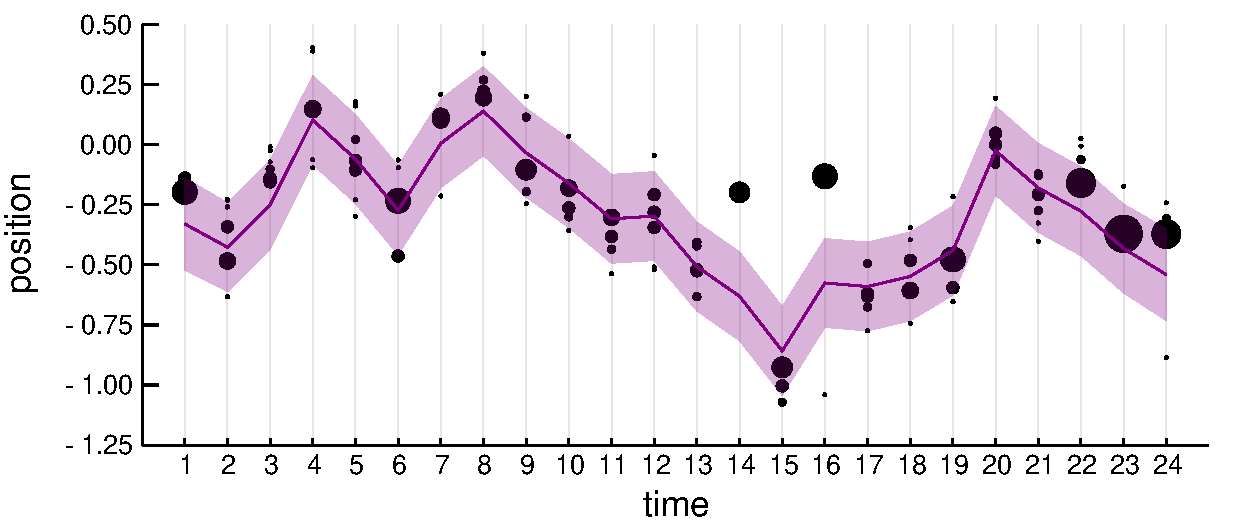
\includegraphics[width=\colwidth]{smc_kalman.pdf}
\caption{Exact posterior (purple) and weighted SMC particles before resampling (black) for a linear Gaussian model.}
\end{figure}
\end{block}

\begin{block}{Ancestral Degeneracy}
However, these particles cannot approximate the smoothing distributions. For that we need a sample of \emph{trajectories} covering all $t$ time steps, not just a sample of particles at each time step.\\[10pt]

We have a sample of $N$ such trajectories: the ancestral trajectories of each of the $N$ particles alive at time $t$.
But due to the resampling mechanism that generates these ancestries, they coalesce backwards in time, leaving much fewer than $N$ distinct samples at time 0. 

%% crop off axis titles
\begin{figure}
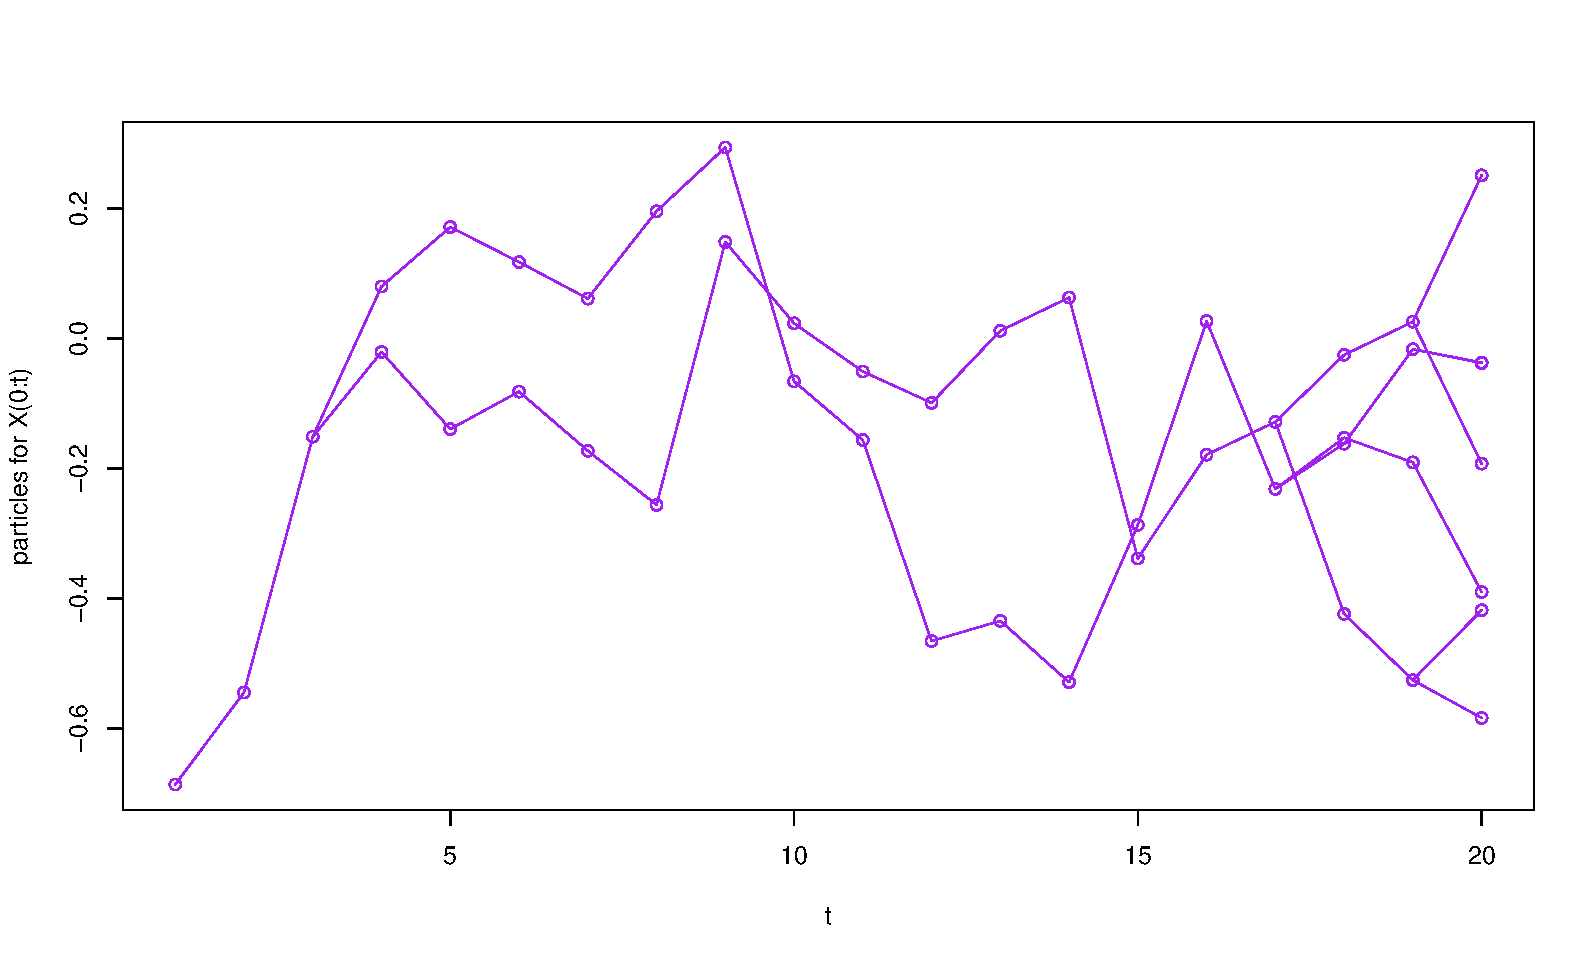
\includegraphics[width=0.9\colwidth]{degeneracy.pdf}
\caption{Trajectories arising from a sample of N=6 particles. Except at the last few time steps there are no more than two distinct lineages.}
\end{figure}

This phenomenon is known as \emph{ancestral degeneracy}. It can be mitigated by changing the resampling procedure, but it cannot be eradicated.

\end{block}
\end{column}

\begin{column}{\colwidth}
\begin{block} %{Kingman Coalescent}

%Viewed backwards in time, the genealogy of the particles is a \emph{coalescent process}. Population genetics provides us with a limiting model which is known to describe the coalescents of a wide class of population models. \\[10pt]
%
%We consider asymptotic behaviour as $N\to\infty$, and choose a suitable time scale which depends on $N$.

\end{block}
\end{column}
\end{columns}

\end{frame}
\end{document}